\documentclass{beamer}
\usepackage[english]{babel}
\usepackage[utf8]{inputenc}
\usepackage{hyperref}
\usepackage{graphicx}
\usepackage{subfig}

\definecolor{links}{HTML}{4a0c80}
\hypersetup{colorlinks,linkcolor=,urlcolor=links}
\usetheme{default}
\usecolortheme{beaver}
\title[Clustering metagenomic contigs]{Clustering metagenomic contigs based on composition and coverage}
\author{Brynjar Smári Bjarnason}
\institute{KTH -- School of Computer Science and Communication}
\date{\today}
\begin{document}

\section{Code}
\begin{frame}
\titlepage
\end{frame}
\begin{frame}{Code}
Go through code
\end{frame}

\section{Results}
\subsection{In silico NCBI contigs}
\begin{frame}{Composition of in silico contigs from NCBI}
Data:
\begin{enumerate}
\item 184 species from 55 genera and 13 families
\item $\approx$100 contigs from genera gave roughly 5.500 contigs
\item 100bp, 1.000bp, 10.000bp
\end{enumerate}
\end{frame}
\begin{frame}{Precision and recall, contig length 10.000, kmer 4 and 5}
\begin{figure}[h]
\centering
\subfloat[][]{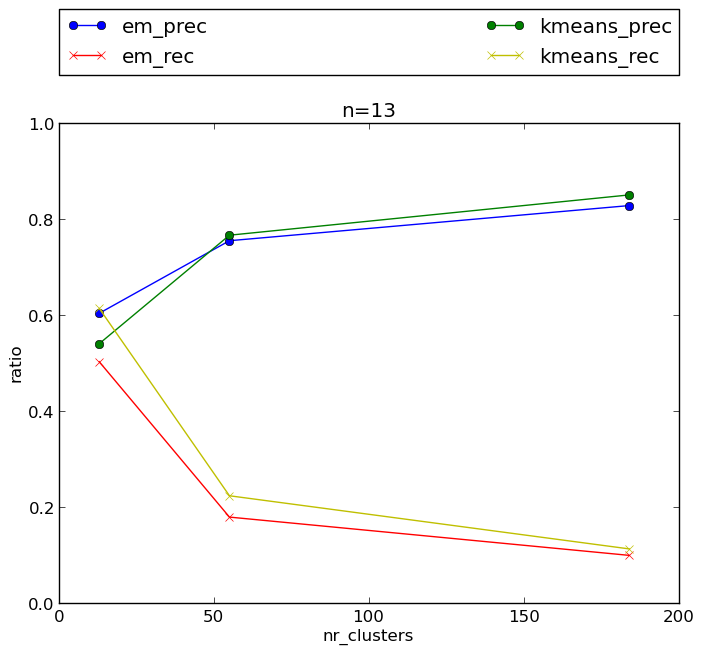
\includegraphics[width=0.3\linewidth]{./contig_10000_k_4_c_13}}
\subfloat[][K=4]{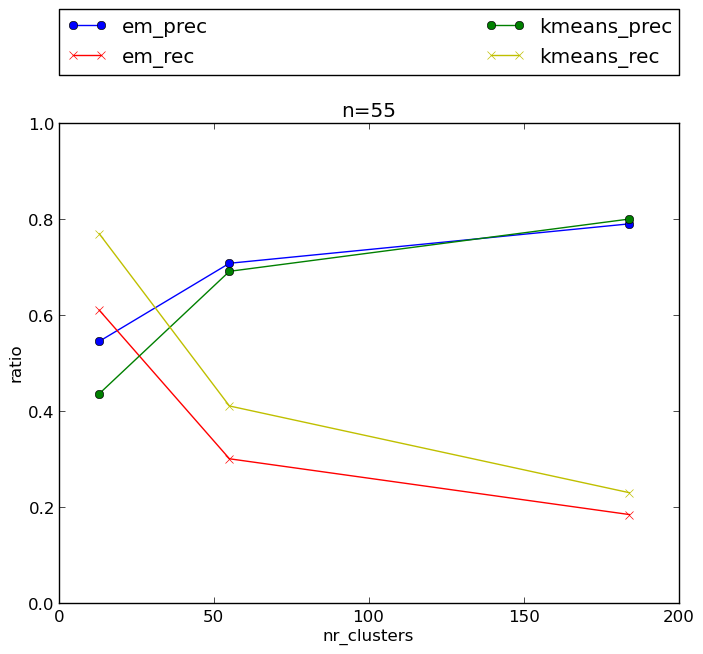
\includegraphics[width=0.3\linewidth]{./contig_10000_k_4_c_55}}
\subfloat[][]{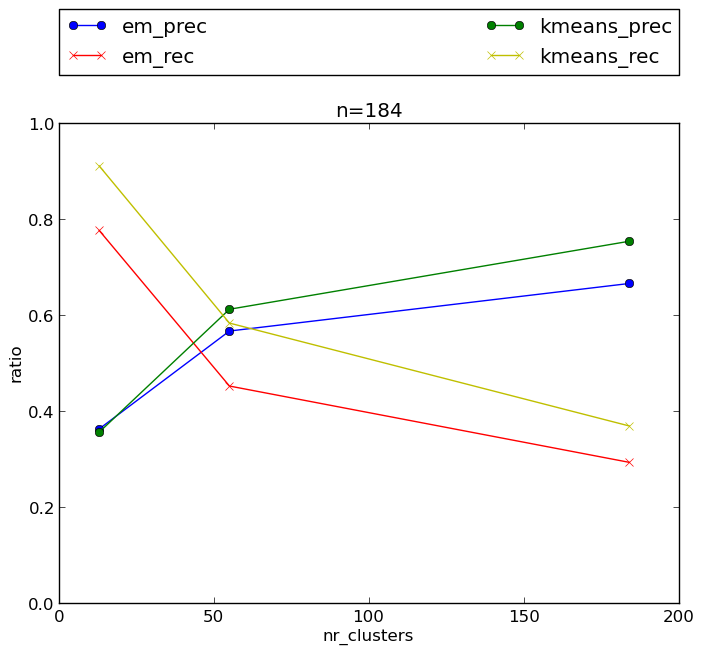
\includegraphics[width=0.3\linewidth]{./contig_10000_k_4_c_184}}
\qquad
\subfloat[][]{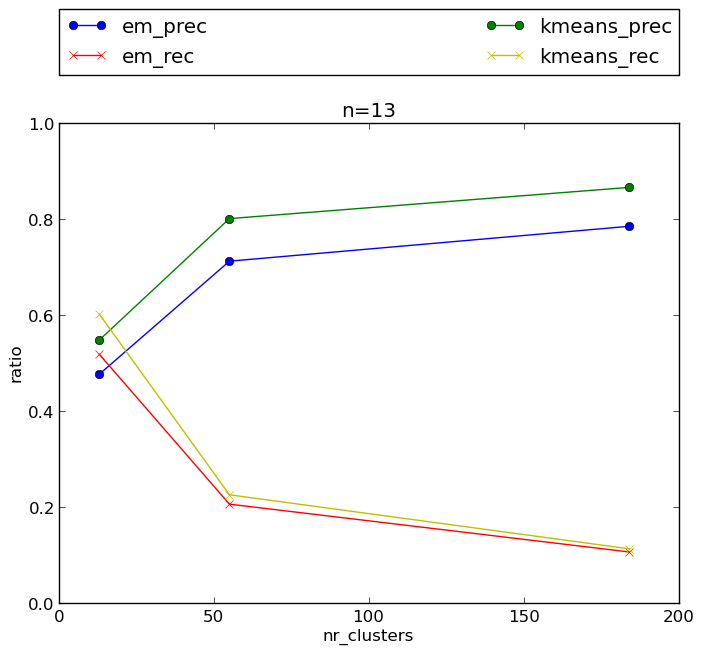
\includegraphics[width=0.3\linewidth]{./contig_10000_k_5_c_13}}
\subfloat[][K=5]{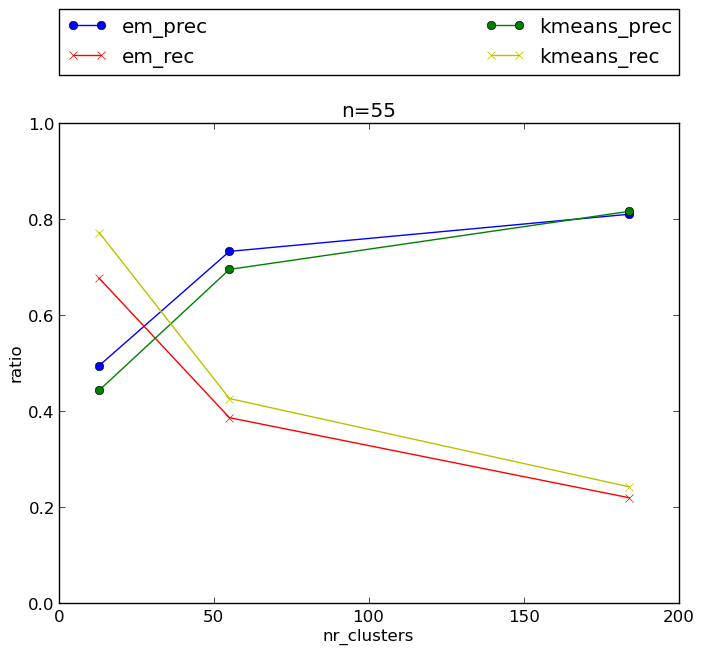
\includegraphics[width=0.3\linewidth]{./contig_10000_k_5_c_55}}
\subfloat[][]{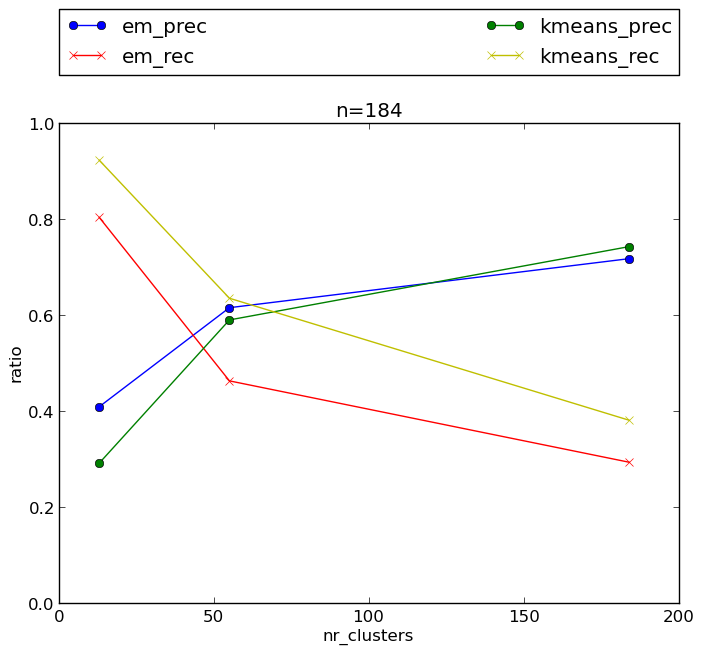
\includegraphics[width=0.3\linewidth]{./contig_10000_k_5_c_184}}
\end{figure}

\end{frame}

\subsection{Mock}
\begin{frame}{Composition of assembled Mock contigs}
\begin{enumerate}
\item 50.000 contigs
\item 40 species
\item 4 kmer length
\end{enumerate}
The results on species level: precision 0.616, recall 0.586
\end{frame}

\begin{frame}{Coverage of in silico Mock timeseries}
\begin{enumerate}
\item 50.000 contigs
\item 40 species
\item 2, 5, 10, 15, 30, 46 samples
\end{enumerate}
\begin{center}
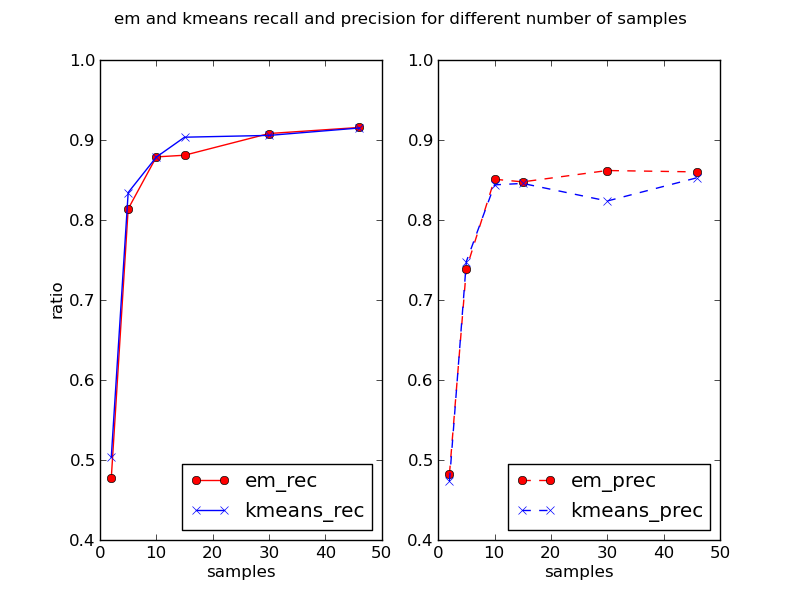
\includegraphics[width=0.7\linewidth]{./coverage-mock}\\
\end{center}
\end{frame}

\section{Code}
\begin{frame}{What needs improvement}
\begin{itemize}
\item One EM and Kmeans for all types of models
\item Joint model for composition and coverage
\item Memory and execution efficiency
\item Estimate number of clusters
\item Different models for composition
\end{itemize}
\end{frame}

\end{document}